\documentclass[10pt,a4paper]{article}
\usepackage[utf8]{inputenc}
\usepackage{polski}
\usepackage{amsmath}
\usepackage{amsfonts}
\usepackage{amssymb}
\usepackage{graphicx}
\usepackage{hyperref}
\usepackage{listings}
\usepackage{color}
\protect\usepackage{ucs}

\author{Klaudia Czuba, Mateusz Koprucki}
\title{VetOS - system wsparcia kliniki weterynaryjnej}
\date{}
\begin{document}

\lstset{columns=fullflexible, basicstyle=\ttfamily,xleftmargin=-2.5cm,frame=lr,framesep=2pt,framerule=0pt,showspaces=false,
inputencoding=utf8x, 
extendedchars=\true,
literate={ą}{{\k{a}}}1
{Ą}{{\k{A}}}1
{ę}{{\k{e}}}1
{Ę}{{\k{E}}}1
{ó}{{\'o}}1
{Ó}{{\'O}}1
{ś}{{\'s}}1
{Ś}{{\'S}}1
{ł}{{\l{}}}1
{Ł}{{\L{}}}1
{ż}{{\.z}}1
{Ż}{{\.Z}}1
{ź}{{\'z}}1
{Ź}{{\'Z}}1
{ć}{{\'c}}1
{Ć}{{\'C}}1
{ń}{{\'n}}1
{Ń}{{\'N}}1}
	\setlength{\topmargin}{-2cm}
\thispagestyle {empty}
\begin{center}
{\LARGE WYŻSZA SZKOŁA ZARZĄDZANIA EDUKACJA}\\[50]








Klaudia Czuba


	Nr albumu 24111
	
	
	Mateusz Koprucki
	
	
	Nr albumu 24081\\[50]
	
	\textbf{Kierunek: Informatyka}\\[50]
	
	{\LARGE \textbf{DOKUMENTACJA PROJEKTOWA SYSTEMU BAZY DANYCH} \\[20]
	
	\textbf{"VetOS - system wsparcia kliniki weterynaryjnej"}}\\[60]
	

\end{center}

\begin{flushright}
	Przedmiot:\\
	\textbf{Projektowanie systemów baz danych}\\[70]
	Prowadzący:\\
	dr inż. Zbigniew Wrona\\[70]
\end{flushright}
\begin{center}
	WROCŁAW 2017
\end{center}

	\newpage
	\tableofcontents
	\newpage
	
	\section{Wstęp}
	Przedmiotem dokumentacji jest system wsparcia kliniki weterynaryjnej przygotowany na zajęcia laboratoryjne z systemów baz danych. Autorami systemu są:
		\begin{itemize}
			\item Klaudia Czuba
			\item Mateusz Koprucki
		\end{itemize}
	System został zaprojektowany w formie aplikacji webowej do stworzenia której użyto następujących technologii:
		\begin{itemize}
			\item Serwer www - Apache2 wraz z PHP
			\item Serwer bazodanowy - Mysql 5.6.15
			\item System zarządzania treścią (CMS) Wordpress 4.7 z rozszerzeniami
		\end{itemize}

	Do celów demonstracyjnych aplikacja posiada trzy konta:
		\begin{itemize}
			\item vet\_test, hasło vet\_test - do prezentacji grupy weterynarzy
			\item staff\_test, hasło staff\_test - do prezentacji grupy obsługi
			\item admin\_test, hasło  admin\_test - do prezentacji możliwości administracji
		\end{itemize}
	W dokumentacji zamieszczono kody źródłowe SQL ze zmiennymi PHP np. 
	\begin{itemize}
		\item '.\$zmienna.'
		\item '\$zmienna'
	\end{itemize}
		
		Pełne repozytorium dostępne jest pod adresem: 
	
	\url{https://github.com/zaknaifen/vetos_core}
	

Plik SQL bazy (vetos\_core\_final.sql):


\url{https://github.com/zaknaifen/vetos_core/tree/master/sql} 
	
	\section{Definicja systemu}
	\subsection{Wymagania biznesowe}
	Wymagania funkcjonalne:
	\begin{itemize}
		\item Aplikacja VetOS nie może wymagać instalacji dodatkowych elementów na komputerach obsługi. Każdy system operacyjny posiada przeglądarkę internetową, co jest jedynym wymaganiem systemowym programu.
		\item System musi posiadać funkcję przypisywania ról do konkretnych użytkowników. 
		\item Użytkownik ma mieć dostęp tylko do sekcji dla niego przenaczonej. 
		\newpage
		\item System powienien posiadać:
			\begin{itemize}
				\item Moduł do obsługi pacjentów
				\item Moduł do zarządzania wizytami
				\item Moduł zamawiania produktów od dostawców
				\item Moduł obsługi zgłoszeń technicznych 
				\item Moduł zarządzania powyższymi elementami
			\end{itemize}
		\item System VetOS musi umożliwiać komunikację z Bazami danych MySQL
		\item Musi istnieć możliwość gromadzenia historii zamówień i historii wizyt.
	\end{itemize}
	Wymagania niefunkcjonalne:
	\begin{itemize}
		\item System musi zapewniać dostępność ciągłą w systemie 24 godziny dziennie, 7 dni w tygodniu.
		\item System musi zapewnić skalowanie, rekonfigurację, osadzanie nowych usług bez zakłócania pracy innych aplikacji i operacji biznesowych.
		\item System musi być intuicyjny w obsłudze.
	\end{itemize}

	\subsection{Cele biznesowe}
	System bazy danych umożliwi usprawnienie procesów obsługi pacjentów, zarządzania zasobami i archiwizacji danych. Dotychczasowo klinika posługiwała się dokumentacją papierową co wpływało negatywnie na jakość gromadzonych danych i wydłużenie procesów obsługi.
	
	Do celów finansowych zalicza się:
	\begin{itemize}
		\item Ograniczenie kosztów magazynowania dokumentacji
		\item Ograniczenie czasu przygotowywania dokumentacji zamówień 
		
	\end{itemize}
	Do celów pozafinansowych zalicza się:
	\begin{itemize}
		\item Łatwość a przez to szybsze wynajdowanie informacji
		\item Odciążenie pracowników kliniki dzięki automatyzacji procesów
	\end{itemize}

	\subsection{Specyfikacja systemu bazy danych}
	System oparty jest na relacyjnej bazie danych, zainstalowany na centralnym serwerze do którego mają dostęp wszystkie komputery w placówcę poprzez serwer WWW.
	
	\section{Zakres i ograniczenia}
	\begin{itemize}
		\item System nie będzie miał dostępu do procesów kadrowo-płacowych. 
		\item System nie będzie posiadał funkcjonalności zewnętrznej tj. części dla pacjentów.
		\item System bez rozbudowy infrastruktury sieciowej będzie systemem lokalnych dla danej placówki.
	\end{itemize}
	


	\section {Instalacja}
		W celu zainstalowania systemu należy zainstalować na serwerze lub komputerze lokalnym środowisko
		\begin{itemize}
			\item Dla Windows: Webserv 2.2
			\item Dla Linux: apache2 z php i mariadb.
		\end{itemize}
	Następnie ściągnąc repozytorium z adresu podanego we wstępie do lokalizacji środowiska. Z folderu sql wgrać poprzez phpmyadmin lub konsole mysql plik sql z bazą danych. 
	
	
	
	
	
	\section {Użytkownicy}
		Aplikacja pozwala na przypisanie do systemu wiele kont przez administrację z podziałem na grupy zdefinowane przez twórców aplikacji. Są to:
		\begin{itemize}
			\item Weterynarz (vet) - grupa przeznaczona dla lekarzy, pozwala na dostęp do modułu weterynaryjnej aplikacji
			\item Obsługa (staff) - grupa przeznaczona dla obsługi z dostępem do sekcji modułu obsługi
			\item Administratcja (admin) - grupa administracyjna, pełen dostęp do modułów. 
		\end{itemize}
	
	\section{Moduły}
	Aplikacja została podzielona na trzy główne moduły. 
	\subsection{Strona główna}
	Po uruchomieniu aplikacji ukazuje się strona główna z wiadomościami i aktualizacjami, w lewym górnym logu widnieje ikona do uruchomienia menu systemu. Dla użytkowników z grupy administracja będzie również widoczny podłużny pasek systemu CMS do zarządzania użytkownikami (tworzenie, modyfikowanie, usuwanie.)
	
	\includegraphics[width=11cm]1
	
	
	\begin{itemize}
		\item SQL wykorzystany dla tej strony:
	\begin{lstlisting}
		SELECT 
			news_tresc as NEWS, 
			news_data as DATA 
		FROM	 
			news 
		order by 
			news_data desc 
		LIMIT 10 ;
	\end{lstlisting}
	
	\end{itemize}

	\subsection{Moduł weterynarza}
	Moduł weterynarza jest dostępny dla użytkowników z grupy weterynarzy i administracji. Sekcja została podzielona na dwie części:
	\begin{itemize}
		\item $[W$] Grafik - przyszłe wizyty weterynarza, wraz z formularzem przejścia do konkretnej wizyty. 
		
		SQL wykorzystany dla tej strony:
		\begin{lstlisting}
		select 
			event_id as `Numer wizyty`,event_begin as `data`,
			event_time as `czas`,patient_id as `numer pacjenta`
		from 
			wp_calendar 
		where 
			vet_id=(select ID 
				from 
				wp_users 
				where user_login="'.$login .'")
		\end{lstlisting}
		
		\includegraphics[width=11cm]2
		
		
		Po wprowadzeniu numeru wizyty aplikacja przenosi użytkownika na stronę realizacji wizyty, gdzie:
			\begin{itemize}
				\item W części górnej pojawiają się dane pacjenta wraz z powodem wizyty
				\item W centralnej części znajduję się arkusz do wypełnienia podczas wizyty
					\begin{itemize}
						\item Diagnoza
						\item Zalecenia
					\end{itemize}
				
			\includegraphics[width=11cm]3
				
		SQL Wykorzystany dla tej strony:	
		\begin{lstlisting}
		select 
			patient_id as `numer pacjenta`, 
			patient_name as `imie pacjenta`, 
			patient_race as `rasa`,
			patient_birthdate as `data urodzenia`
		from 
			patient_info 
		where 
			patient_id=(select patient_id 
			from wp_calendar where event_id='.$visit_id.');
			
		---------------------------------------------------
		select 
			patient_health_card_id as `nr`,
			patient_health_card_date as `data`,
			patient_health_card_desc as `diagnoza`,
			patient_health_card_recom as `zalecenia`
		from 
			patient_health_card 
		where 
			patient_health_card_patient_id=(select patient_id 
				from wp_calendar 
				where event_id='.$visit_id.') 
		order by patient_health_card_date desc LIMIT 4;
		---------------------------------------------------
		SELECT 
			count(patient_health_card_id) 
		FROM 
			patient_health_card 
		where 
			patient_health_card_patient_id=(select patient_id 
				from wp_calendar 
				where event_id='.$visit_id.');
		---------------------------------------------------
		INSERT INTO 
			patient_health_card
			(patient_health_card_patient_id,
		 	patient_health_card_desc, 
		 	patient_health_card_recom, 
		 	patient_health_card_addby) 
		VALUES 
			((select patient_id 
				from wp_calendar 
				where event_id=18),
			'$visit_diag',
			'$visit_rec',
			'$login');
		
		
		
		
		\end{lstlisting}
		
			
				
				
				\item Z prawej strony wyświetlają się 4 ostatnie wpisy z historii wizyt pacjenta z możliwością przejścia do pełnej historii.
				
				
				\includegraphics[width=11cm]5
			
			\end{itemize}
	
		
		
		SQL Wykorzystany dla tej strony:
		
		\begin{lstlisting}
		select 
			a.vet_id,
			a.event_id as `numer wizyty`,
			a.event_begin as `data`,
			a.event_time as `godzina`,
			a.event_desc as `opis`,
			b.patient_id as `numer pacjenta`,
			b.patient_name as `imie pacjenta`,
			c.owner_name as `imie  wlasciciela`,
			c.owner_surname as `nazwisko wlasciciela`
		from 
			wp_calendar a
		join 
			patient_info b 
			on a.patient_id=b.patient_id
		join 
			owner_info c 
			on b.patient_id=c.owner_id
		where 
			(event_time>=curtime() 
			and a.vet_id=(select ID from wp_users 
		  		where user_login="'.$login.'") 
			and event_begin>=curdate())
		or 
			(event_begin>=sysdate()
			and a.vet_id=(select ID from wp_users
		  		where user_login="'.$login.'"))
		order by event_begin asc;
		\end{lstlisting}
		
		
		
		
		\item $[W$] Spis wizyt - strona pokazuje wszystkie wizyty przypisane do weterynarza, zarówno te przeszłe jak i przyszłe. 
	
		
		\includegraphics[width=11cm]4
		
		
		SQL Wykorzystany dla tej strony:
		\begin{lstlisting}
		select 
			event_id as `Numer wizyty`,
			event_begin as `data`,
			event_time as `czas`,
			patient_id as `numer pacjenta`
		from 
			wp_calendar where vet_id=(select ID 
				from wp_users 
				where user_login="'.$login.'")  
		order by event_begin  asc;
		\end{lstlisting}
			\end{itemize}
	\newpage	
	\subsection{Moduł obsługi}	
		Moduł przeznaczony dla personelu odpowiedzialnego za zamówienia towarów, dodawania pacjentów i umawiania bądź ich anulacji. Sekcja została podzielona na cztery części. 
		
		\begin{itemize}
			\item $[S$] Wizyty - sekcja podzielona jest na 3 częsci:
			\begin{itemize}
				\item Kalendarz z podglądem dodanych wizyt.
				\item Formularze dodawania i anulowania wizyt oraz wyszukiwanie danych pacjentów.
				\item Listy dostępnych lekarzy.
			\end{itemize}
				\includegraphics[width=11cm]6
				
			
			SQL Wykorzystany dla tej strony:
			\begin{lstlisting}
			insert 
			into 
				wp_calendar 
				(event_begin,
				event_end,patient_id,event_title, event_desc, 
				event_time,event_recur,event_repeats,event_author,
				vet_id, event_active ) 
			values 	
				('$new_visit_date','$new_visit_date',
				'$new_visit_patient','Wizyta',
				'$new_visit_desc','$new_visit_time',
				'S','0','1','$new_visit_vet','1');
			---------------------------------------------------
			delete 
				from wp_calendar
			WHERE 
				event_id='$visit_number';
			\end{lstlisting}	
				
				
			
			
			 \item $[S$] Dodaj pacjenta - sekcja podzielona jest na 2 części:
			 \begin{itemize}
			 	\item Formularze dodawania właściciela i pacjenta.
			 	\item Formularz wyszukiwania danych właściciela, jeżeli już wcześniej się zarejestrował a dodaje kolejnego podopiecznego do systemu.
			 	
			 \includegraphics[width=11cm]7
			
			 \end{itemize}
		 SQL Wykorzystany dla tej strony:
\begin{lstlisting}
		INSERT 
			INTO patient_info 
		SET patient_name='$npn', patient_race='$npr',
			patient_birthdate='$npbd', patient_owner_id='$npoi',
		    patient_addby='$login' 	 
		--------------------------------------------------- 
		SELECT 
			patient_id 
		FROM 
			patient_info 
		where 
			patient_addby="'. $login .'" 
		ORDER BY patient_id DESC LIMIT 1;	 
		---------------------------------------------------
		INSERT INTO owner_info 
		SET 
			owner_name='$non', owner_surname='$nos', 
			owner_phone='$nop', owner_address='$noa', 
			owner_addby='$login' "\end{lstlisting}	 
			 \item $[S$] Karta właściciela - sekcja wyświetla wszystkie dane właściciela oraz jego zwierząt
			 
			 \includegraphics[width=11cm]8
		
		SQL wykorzystany dla tej strony:
		\begin{lstlisting}
		select
			owner_id as `numer właściciela`, 
			owner_name as `imie`, 
			owner_surname as `nazwisko`, 
			owner_phone as `numer telefonu`, 
			owner_address as `adres` 
		from owner_info 
		where 
			owner_id="'. $owner_id . '" 
			or owner_surname="'. $owner_surname . '"
		---------------------------------------------------
		select 
			patient_id as `numer pacjenta`, 
			patient_name as `imie`, 
			patient_race as `rasa`, 
			patient_birthdate as `data urodzenia` 
		from owner_info a
		join patient_info b
		on a.owner_id=b.patient_owner_id
		where 
			owner_id="'. $owner_id . '" 
			or owner_surname="'. $owner_surname . '";
		\end{lstlisting}
			 
			 \newpage
			 \item $[S$] Dostępne materiały - sekcja przeznaczona do zamawiania towarów z dostępnej listy. Strona została podzielona na dwie części:
			 	\begin{itemize}
			 		\item Spis produktów
			 		\item Formularz dodawania i usuwania produktów do zamówienia i wysyłania gotowego zamówienia.
			 	\end{itemize}
		 	\includegraphics[width=11cm]9
		 	
		 SQL wykorzystany dla tej strony:
		 
		\begin{lstlisting}
		select 
			w.warehouse_id as `numer dostawcy`,
			s.warehouse_stock_id as `numer produktu`,
			i.warehouse_name as `nazwa`,
			s.warehouse_stock_name as `nazwa towaru`,
			s.warehouse_stock_desc as `opis`,
			s.warehouse_stock_value as `cena`,
			s.warehouse_stock_quant as `ilość w opakowaniu`
		from warehouse w
			join warehouse_info i 
				on w.warehouse_info_ID=i.warehouse_info_id
			join warehouse_stock s 
				on w.warehouse_info_ID=s.warehouse_id
		where warehouse_active="YES";
		---------------------------------------------------
		truncate vetos_core.order;
		---------------------------------------------------
		insert 
			into vetos_core.order_history 
				(order_id, warehouse_id,product_id,
				quantity,order_date,order_by) 
		select * from vetos_core.order;
		---------------------------------------------------
		INSERT 
		INTO vetos_core.order 
		SET 
			warehouse_id='$nov', product_id='$noa',  
			quantity='$noq', order_time='$time', order_by='$login'; 
		---------------------------------------------------
		delete from vetos_core.order 
			order by order_id desc limit 1;
		
		
		\end{lstlisting} 
		 
		 
		\end{itemize}
\subsection {Moduł administracji}
Sekcja została podzielona na sześć części:
	\begin{itemize}
		\item $[A$] Przeglądaj zgłoszenia - strona odpowiedzialna za wyświetlanie aktualnie otwartych zgłoszeń technicznych. Na dole strony znajduje się formularz przejścia do konkretnego zgłoszenia po wpisaniu numeru porządkowego zgłoszenia.
		
		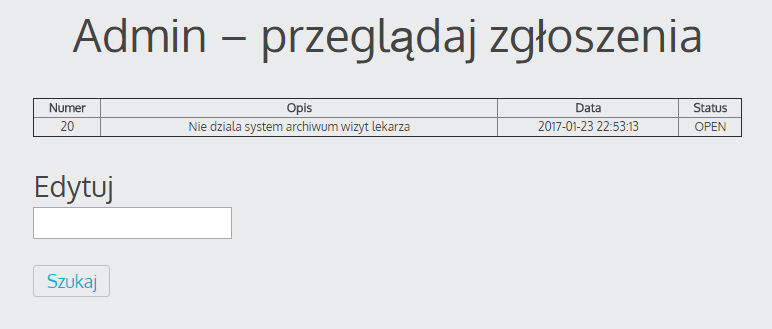
\includegraphics[width=11cm]{10}
		
		SQL wykorzystany dla tej strony:
		\begin{lstlisting}
		select 
			INC_id as Numer, 
			INC_description as Opis, 
			INC_date as Data, 
			INC_status as Status 
		from 
			incidents_main 
		where  
			INC_status="OPEN";
		\end{lstlisting}
		\newpage
		\item $[A$] Szukaj zgłoszenie - formularz do wyszukiwania, wyświetlania i edycji zgłoszeń zarówno otwartych jak i zamkniętych.
		
			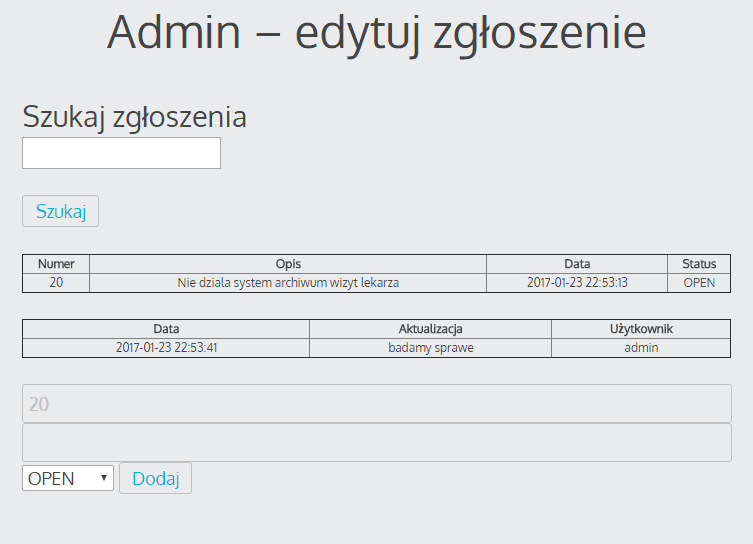
\includegraphics[width=11cm]{11}
		
		SQL wykorzystany dla tej strony:
		\begin{lstlisting}
		select 
			INC_id as Numer, 
			INC_description as Opis, 
			INC_date as Data, 
			INC_status as Status 
		from 
			incidents_main 
		where 
			INC_id='. $ticket . ';
		---------------------------------------------------
		SELECT 
			b.incidents_log_time as Data, 
			b.incidents_log_text as Aktualizacja, 
			b.incidents_log_user as Użytkownik 
		FROM 
			incidents_main a 
		INNER JOIN 
			incidents_log b 
			ON a.INC_id=b.incidents_log_ticket 
		where 
			a.INC_id='. $ticket . ' 
		order by 
			b.incidents_log_time ASC; 
		---------------------------------------------------
		INSERT INTO 
			incidents_log 
		SET 
			incidents_log_user='$login', 
			incidents_log_text='$ticket_desc', 
			incidents_log_ticket='$ticket', 
			incidents_log_time='$created_date' 
		---------------------------------------------------
		UPDATE 
			incidents_main 
		SET 
			INC_status = '$ticket_desc_status' 
		where 
			INC_id='$ticket'
		\end{lstlisting}
		
		
		\item $[A$] Archiwum zgłoszeń - strona wyświetlająca wszystkie zamknięte zgłoszenia. Na górze strony znajduje się formularz wyszukania zgłoszenia.
		
	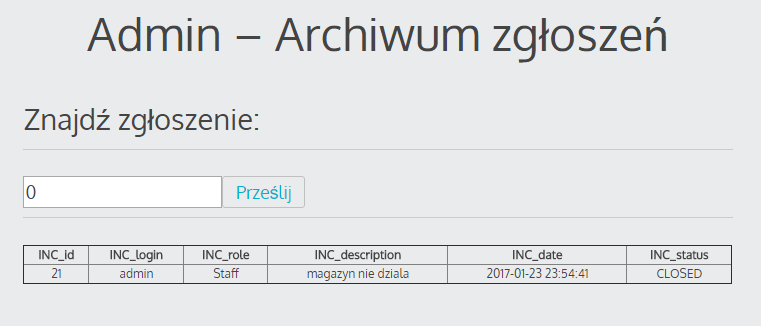
\includegraphics[width=11cm]{12}
		
		SQL wykorzystany dla tej strony:
		\begin{lstlisting}
		select 
			INC_id,INC_login,
			INC_role,INC_description,
			INC_date,INC_status 
		from 
			incidents_main 
		where INC_status="CLOSED" 
		LIMIT 30;
		\end{lstlisting}
		
		\item $[A$] Dodaj news - strona zawiera formularz dodawania wiadomości do głównej strony. 
		
		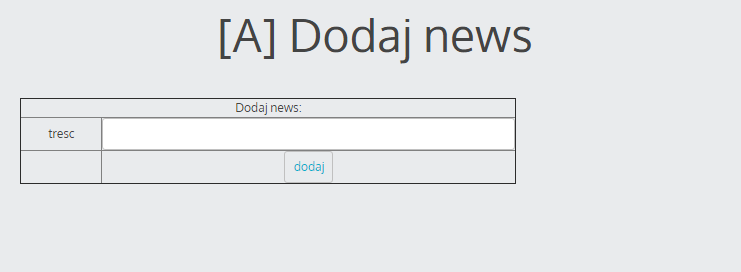
\includegraphics[width=11cm]{13}
		\newpage
			SQL wykorzystany dla tej strony:
		\begin{lstlisting}
		INSERT INTO 
			news 
		SET 
			news_tresc='$nn'; 
		\end{lstlisting}
		
		\item $[A$] Dostawcy - strona wyświetlająca wszystkich dostawców dla kliniki. 
		
		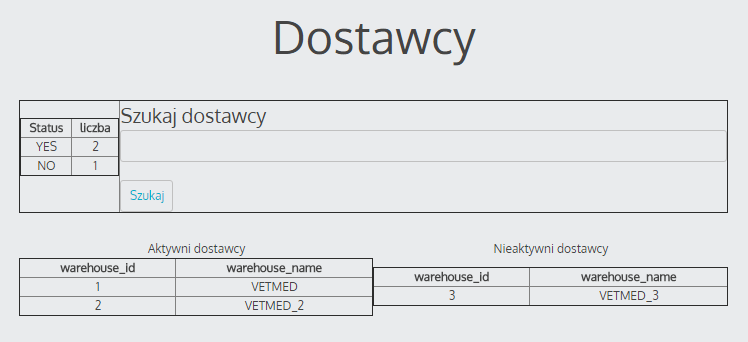
\includegraphics[width=11cm]{14}
		
		Sekcja została podzielona na dwie części:
			\begin{itemize}
				\item Formularz wyszukania dostawcy i przejścia do jego edycji (aktywacji bądź deaktywacji dostawcy oraz usunięcia dostępnego produktu z listy dostawcy).
					
					
				
				\item Podsumownia aktywnych i nieaktywnych dostawców
				\end{itemize}
		
		SQL wykorzystany dla tej strony:
		\begin{lstlisting}
		select 
			warehouse_active as Status,
			count(*) as liczba 
		from 
			warehouse 
		group by 
			warehouse_active desc;
		
		select 
			a.warehouse_id,
			b.warehouse_name 
		from 
			warehouse a 
		inner 
			join warehouse_info b 
			on a.warehouse_info_ID=b.warehouse_info_id 
		where 
			a.warehouse_active="YES";
		---------------------------------------------------
		select 
			a.warehouse_id,
			b.warehouse_name 
		from 
			warehouse a 
		inner join 
			warehouse_info b 
			on a.warehouse_info_ID=b.warehouse_info_id 
		where 
			a.warehouse_active="NO";
		---------------------------------------------------
		delete from 
			warehouse_stock 
		where 
			warehouse_stock_id='$dav';
		---------------------------------------------------
		select 
			warehouse_name as nazwa , 
			warehouse_city as miasto , 
			warehouse_address as adres , 
			warehouse_tel as telefon 
		from 
			warehouse_info 
		where 
			warehouse_info_id='. $supplier . ' ;
		---------------------------------------------------
		SELECT 
			warehouse_stock_id as numer, 
			warehouse_stock_name as nazwa, 
			warehouse_stock_desc as opis, 
			warehouse_stock_value as cena, 
			warehouse_stock_quant as ilosc 
		from 
			warehouse_stock 
		where 
			warehouse_id='. $supplier . ' ; 
		---------------------------------------------------
		UPDATE 
			warehouse 
		SET 
			warehouse_active='$warehouse_status' 
		WHERE 
			warehouse_id='$supplier' 
		
		
		\end{lstlisting}
		\newpage
		
		\item $[A$] Dodaj artykuł - strona odpowiedzialna za dodawania nowych artykułów do dostawców w systemie. Sekcja została podzielona na dwie części:
		
			\begin{itemize}
				\item Formularz dodania nowego produktu
				\item Listy aktywnych dostawców
			\end{itemize}
		
	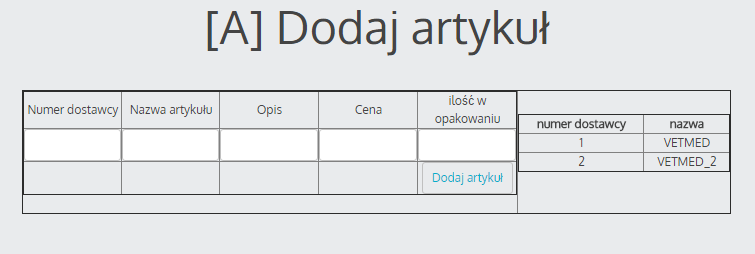
\includegraphics[width=11cm]{15}
		
		SQL wykorzystany dla tej strony:
		\begin{lstlisting}
		INSERT INTO 
			warehouse_stock 
		SET 
			warehouse_id='$nwsi', 
			warehouse_stock_name='$nwsa',  
			warehouse_stock_desc='$nwsd', 
			warehouse_stock_value='$nwsv', 
			warehouse_stock_quant='$nwsq' 
		---------------------------------------------------
		select 
			a.warehouse_id as `numer dostawcy`,
			b.warehouse_name as `nazwa`
		from 
			warehouse a 
		join 
			warehouse_info b 
			on a.warehouse_info_ID=b.warehouse_info_id 
		where 
			a.warehouse_active="YES";
		\end{lstlisting}
		
	\end{itemize}

\subsection{Moduł zgłoszeń}
	Moduł odpowiedzialny za dodawanie i przeglądanie zgłoszeń technicznych dla użytkowników końcowych systemu. Strona została podzielona na cztery części:
	\begin{itemize}
		\item Szukaj zgłoszenia - formularz wyszukania i wyświetlenia szczegółów zgłoszenia
		\item Aktualne zgłosenia - lista otwartych zgłoszeń użytkownika
		\item Zamknięte zgłoszenia - lista zamkniętych zgłoszeń
		\item Formularz dodania nowego zgłoszenia
	\end{itemize}

	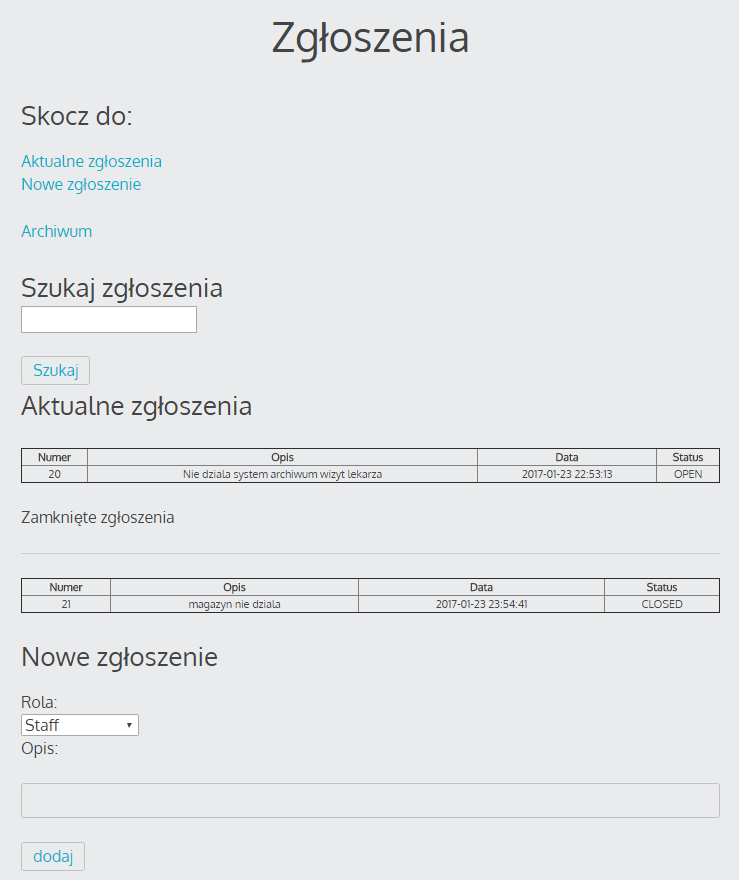
\includegraphics[width=11cm]{16}
	
	SQL wykorzystany dla tej strony:
	\begin{lstlisting}
	select 
		INC_id as Numer, 
		INC_description as Opis, 
		INC_date as Data, 
		INC_status as Status 
	from 
		incidents_main 
	where 
		INC_login="'. $login . '" 
		and INC_status="OPEN"; 
	---------------------------------------------------
	select 
		INC_id as Numer, 
		INC_description as Opis, 
		INC_date as Data, 
		INC_status as Status 
	from 
		incidents_main 
	where 
		INC_login="'. $login . '" 
		and INC_status="CLOSED"; 
	---------------------------------------------------
	INSERT INTO 
		incidents_main 
	SET 
		INC_login='$login', 
		INC_role='$role', 
		INC_description='$desc', 
		INC_date='$created_date', 
		INC_status='OPEN'; 
	
	
	\end{lstlisting}
\section{Projektowanie fizyczne}
	\begin{lstlisting}
	SET SQL_MODE = "NO_AUTO_VALUE_ON_ZERO";
	SET time_zone = "+00:00";
	CREATE DATABASE IF NOT EXISTS `vetos_core` DEFAULT CHARACTER SET utf8 COLLATE utf8_general_ci;
	USE `vetos_core`;
	
	DROP TABLE IF EXISTS `incidents_log`;
	CREATE TABLE IF NOT EXISTS `incidents_log` (
	`incidents_log_id` int(11) NOT NULL AUTO_INCREMENT,
	`incidents_log_time` timestamp NULL DEFAULT NULL,
	`incidents_log_text` varchar(500) DEFAULT NULL,
	`incidents_log_user` varchar(100) DEFAULT NULL,
	`incidents_log_ticket` int(11) DEFAULT NULL,
	PRIMARY KEY (`incidents_log_id`)
	) ENGINE=InnoDB  DEFAULT CHARSET=utf8 AUTO_INCREMENT=4 ;
	
	DROP TABLE IF EXISTS `incidents_main`;
	CREATE TABLE IF NOT EXISTS `incidents_main` (
	`INC_id` int(11) NOT NULL AUTO_INCREMENT,
	`INC_login` varchar(255) NOT NULL,
	`INC_role` varchar(255) DEFAULT NULL,
	`INC_description` varchar(255) DEFAULT NULL,
	`INC_date` timestamp NOT NULL DEFAULT CURRENT_TIMESTAMP ON UPDATE CURRENT_TIMESTAMP,
	`INC_status` varchar(255) DEFAULT NULL,
	`INC_user` varchar(255) DEFAULT NULL,
	`inc_close_date` timestamp NULL DEFAULT NULL,
	`INC_resolution` varchar(500) DEFAULT NULL,
	PRIMARY KEY (`INC_id`)
	) ENGINE=InnoDB  DEFAULT CHARSET=utf8 AUTO_INCREMENT=22 ;
	
	DROP TABLE IF EXISTS `news`;
	CREATE TABLE IF NOT EXISTS `news` (
	`news_id` int(11) NOT NULL AUTO_INCREMENT,
	`news_data` timestamp NULL DEFAULT CURRENT_TIMESTAMP,
	`news_tresc` varchar(800) DEFAULT NULL,
	PRIMARY KEY (`news_id`)
	) ENGINE=InnoDB  DEFAULT CHARSET=utf8 AUTO_INCREMENT=18 ;
	
	DROP TABLE IF EXISTS `order`;
	CREATE TABLE IF NOT EXISTS `order` (
	`order_id` int(11) NOT NULL AUTO_INCREMENT,
	`warehouse_id` int(11) NOT NULL,
	`product_id` int(11) DEFAULT NULL,
	`quantity` int(11) DEFAULT NULL,
	`order_time` date NOT NULL,
	`order_by` varchar(255) NOT NULL,
	PRIMARY KEY (`order_id`)
	) ENGINE=InnoDB  DEFAULT CHARSET=utf8 AUTO_INCREMENT=2 ;
	
	DROP TABLE IF EXISTS `order_history`;
	CREATE TABLE IF NOT EXISTS `order_history` (
	`order_history_id` int(11) NOT NULL AUTO_INCREMENT,
	`order_id` int(11) NOT NULL,
	`warehouse_id` int(11) NOT NULL,
	`product_id` int(11) NOT NULL,
	`quantity` int(11) NOT NULL,
	`order_date` date NOT NULL,
	`order_by` varchar(255) NOT NULL,
	PRIMARY KEY (`order_history_id`)
	) ENGINE=InnoDB  DEFAULT CHARSET=utf8 AUTO_INCREMENT=18 ;
	
	DROP TABLE IF EXISTS `owner_info`;
	CREATE TABLE IF NOT EXISTS `owner_info` (
	`owner_id` int(11) NOT NULL AUTO_INCREMENT,
	`owner_name` varchar(500) DEFAULT NULL,
	`owner_surname` varchar(500) DEFAULT NULL,
	`owner_phone` varchar(500) DEFAULT NULL,
	`owner_address` varchar(500) DEFAULT NULL,
	`owner_info` varchar(500) DEFAULT NULL,
	`owner_addby` varchar(255) NOT NULL,
	PRIMARY KEY (`owner_id`)
	) ENGINE=InnoDB  DEFAULT CHARSET=utf8 AUTO_INCREMENT=7 ;
	
	DROP TABLE IF EXISTS `patient_health_card`;
	CREATE TABLE IF NOT EXISTS `patient_health_card` (
	`patient_health_card_id` int(11) NOT NULL AUTO_INCREMENT,
	`patient_health_card_patient_id` int(11) NOT NULL,
	`patient_health_card_desc` varchar(2000) NOT NULL,
	`patient_health_card_recom` varchar(600) NOT NULL,
	`patient_health_card_date` timestamp NOT NULL DEFAULT CURRENT_TIMESTAMP,
	`patient_health_card_prescription_id` int(11) NOT NULL,
	`patient_health_card_addby` varchar(300) NOT NULL,
	PRIMARY KEY (`patient_health_card_id`)
	) ENGINE=InnoDB  DEFAULT CHARSET=utf8 AUTO_INCREMENT=2 ;
	
	DROP TABLE IF EXISTS `patient_info`;
	CREATE TABLE IF NOT EXISTS `patient_info` (
	`patient_id` int(11) NOT NULL AUTO_INCREMENT,
	`patient_name` varchar(500) DEFAULT NULL,
	`patient_race` varchar(500) DEFAULT NULL,
	`patient_birthdate` date DEFAULT NULL,
	`patient_owner_id` int(11) DEFAULT NULL,
	`patient_info` varchar(500) DEFAULT NULL,
	`patient_addby` varchar(255) NOT NULL,
	PRIMARY KEY (`patient_id`)
	) ENGINE=InnoDB  DEFAULT CHARSET=utf8 AUTO_INCREMENT=6 ;
	
	DROP TABLE IF EXISTS `test_inc`;
	CREATE TABLE IF NOT EXISTS `test_inc` (
	`id` int(11) NOT NULL AUTO_INCREMENT,
	`imie` varchar(100) NOT NULL DEFAULT '',
	`email` varchar(100) NOT NULL DEFAULT '',
	PRIMARY KEY (`id`)
	) ENGINE=InnoDB  DEFAULT CHARSET=utf8 AUTO_INCREMENT=2 ;
	
	DROP TABLE IF EXISTS `warehouse`;
	CREATE TABLE IF NOT EXISTS `warehouse` (
	`warehouse_id` int(11) NOT NULL AUTO_INCREMENT,
	`warehouse_info_ID` int(11) DEFAULT NULL,
	`warehouse_active` varchar(3) DEFAULT 'NO',
	PRIMARY KEY (`warehouse_id`)
	) ENGINE=InnoDB  DEFAULT CHARSET=utf8 AUTO_INCREMENT=4 ;
	
	DROP TABLE IF EXISTS `warehouse_info`;
	CREATE TABLE IF NOT EXISTS `warehouse_info` (
	`warehouse_info_id` int(11) NOT NULL AUTO_INCREMENT,
	`warehouse_name` varchar(100) NOT NULL,
	`warehouse_city` varchar(100) DEFAULT NULL,
	`warehouse_address` varchar(200) DEFAULT NULL,
	`warehouse_tel` varchar(20) DEFAULT NULL,
	PRIMARY KEY (`warehouse_info_id`),
	UNIQUE KEY `warehouse_id` (`warehouse_info_id`)
	) ENGINE=InnoDB  DEFAULT CHARSET=utf8 AUTO_INCREMENT=4 ;
	
	DROP TABLE IF EXISTS `warehouse_stock`;
	CREATE TABLE IF NOT EXISTS `warehouse_stock` (
	`warehouse_stock_id` int(11) NOT NULL AUTO_INCREMENT,
	`warehouse_id` int(11) DEFAULT NULL,
	`warehouse_stock_name` varchar(500) DEFAULT NULL,
	`warehouse_stock_desc` varchar(500) DEFAULT NULL,
	`warehouse_stock_value` int(11) DEFAULT NULL,
	`warehouse_stock_quant` int(11) DEFAULT NULL,
	`warehouse_stock_info` varchar(500) DEFAULT NULL,
	PRIMARY KEY (`warehouse_stock_id`)
	) ENGINE=InnoDB  DEFAULT CHARSET=utf8 AUTO_INCREMENT=6 ;
	
	DROP TABLE IF EXISTS `wp_calendar`;
	CREATE TABLE IF NOT EXISTS `wp_calendar` (
	`event_id` int(11) NOT NULL AUTO_INCREMENT,
	`event_begin` date NOT NULL,
	`event_end` date NOT NULL,
	`patient_id` int(11) NOT NULL,
	`vet_id` int(11) NOT NULL,
	`event_title` varchar(30) COLLATE utf8_unicode_ci NOT NULL,
	`event_desc` text COLLATE utf8_unicode_ci NOT NULL,
	`event_time` time DEFAULT NULL,
	`event_recur` char(1) COLLATE utf8_unicode_ci DEFAULT NULL,
	`event_repeats` int(3) DEFAULT NULL,
	`event_author` bigint(20) unsigned DEFAULT NULL,
	`event_category` bigint(20) unsigned NOT NULL DEFAULT '1',
	`event_link` text COLLATE utf8_unicode_ci,
	`event_active` int(11) NOT NULL,
	PRIMARY KEY (`event_id`)
	) ENGINE=InnoDB  DEFAULT CHARSET=utf8 COLLATE=utf8_unicode_ci AUTO_INCREMENT=25 ;
	
	DROP TABLE IF EXISTS `wp_calendar_categories`;
	CREATE TABLE IF NOT EXISTS `wp_calendar_categories` (
	`category_id` int(11) NOT NULL AUTO_INCREMENT,
	`category_name` varchar(30) COLLATE utf8_unicode_ci NOT NULL,
	`category_colour` varchar(30) COLLATE utf8_unicode_ci NOT NULL,
	PRIMARY KEY (`category_id`)
	) ENGINE=InnoDB  DEFAULT CHARSET=utf8 COLLATE=utf8_unicode_ci AUTO_INCREMENT=2 ;
	
	DROP TABLE IF EXISTS `wp_calendar_config`;
	CREATE TABLE IF NOT EXISTS `wp_calendar_config` (
	`config_item` varchar(30) COLLATE utf8_unicode_ci NOT NULL,
	`config_value` text COLLATE utf8_unicode_ci NOT NULL,
	PRIMARY KEY (`config_item`)
	) ENGINE=InnoDB DEFAULT CHARSET=utf8 COLLATE=utf8_unicode_ci;
	
	DROP TABLE IF EXISTS `wp_cimy_uef_data`;
	CREATE TABLE IF NOT EXISTS `wp_cimy_uef_data` (
	`ID` bigint(20) NOT NULL AUTO_INCREMENT,
	`USER_ID` bigint(20) NOT NULL,
	`FIELD_ID` bigint(20) NOT NULL,
	`VALUE` text COLLATE utf8mb4_unicode_520_ci NOT NULL,
	PRIMARY KEY (`ID`),
	KEY `USER_ID` (`USER_ID`),
	KEY `FIELD_ID` (`FIELD_ID`)
	) ENGINE=InnoDB DEFAULT CHARSET=utf8mb4 COLLATE=utf8mb4_unicode_520_ci AUTO_INCREMENT=1 ;
	
	DROP TABLE IF EXISTS `wp_cimy_uef_fields`;
	CREATE TABLE IF NOT EXISTS `wp_cimy_uef_fields` (
	`ID` bigint(20) NOT NULL AUTO_INCREMENT,
	`F_ORDER` bigint(20) NOT NULL,
	`FIELDSET` bigint(20) NOT NULL DEFAULT '0',
	`NAME` varchar(20) COLLATE utf8mb4_unicode_520_ci DEFAULT NULL,
	`LABEL` text COLLATE utf8mb4_unicode_520_ci,
	`DESCRIPTION` text COLLATE utf8mb4_unicode_520_ci,
	`TYPE` varchar(20) COLLATE utf8mb4_unicode_520_ci DEFAULT NULL,
	`RULES` text COLLATE utf8mb4_unicode_520_ci,
	`VALUE` text COLLATE utf8mb4_unicode_520_ci,
	PRIMARY KEY (`ID`),
	KEY `F_ORDER` (`F_ORDER`),
	KEY `NAME` (`NAME`)
	) ENGINE=InnoDB DEFAULT CHARSET=utf8mb4 COLLATE=utf8mb4_unicode_520_ci AUTO_INCREMENT=1 ;
	
	DROP TABLE IF EXISTS `wp_cimy_uef_wp_fields`;
	CREATE TABLE IF NOT EXISTS `wp_cimy_uef_wp_fields` (
	`ID` bigint(20) NOT NULL AUTO_INCREMENT,
	`F_ORDER` bigint(20) NOT NULL,
	`NAME` varchar(20) COLLATE utf8mb4_unicode_520_ci DEFAULT NULL,
	`LABEL` text COLLATE utf8mb4_unicode_520_ci,
	`DESCRIPTION` text COLLATE utf8mb4_unicode_520_ci,
	`TYPE` varchar(20) COLLATE utf8mb4_unicode_520_ci DEFAULT NULL,
	`RULES` text COLLATE utf8mb4_unicode_520_ci,
	`VALUE` text COLLATE utf8mb4_unicode_520_ci,
	PRIMARY KEY (`ID`),
	KEY `F_ORDER` (`F_ORDER`),
	KEY `NAME` (`NAME`)
	) ENGINE=InnoDB DEFAULT CHARSET=utf8mb4 COLLATE=utf8mb4_unicode_520_ci AUTO_INCREMENT=1 ;
	
	DROP TABLE IF EXISTS `wp_commentmeta`;
	CREATE TABLE IF NOT EXISTS `wp_commentmeta` (
	`meta_id` bigint(20) unsigned NOT NULL AUTO_INCREMENT,
	`comment_id` bigint(20) unsigned NOT NULL DEFAULT '0',
	`meta_key` varchar(255) COLLATE utf8mb4_unicode_520_ci DEFAULT NULL,
	`meta_value` longtext COLLATE utf8mb4_unicode_520_ci,
	PRIMARY KEY (`meta_id`),
	KEY `comment_id` (`comment_id`),
	KEY `meta_key` (`meta_key`(191))
	) ENGINE=InnoDB DEFAULT CHARSET=utf8mb4 COLLATE=utf8mb4_unicode_520_ci AUTO_INCREMENT=1 ;
	
	DROP TABLE IF EXISTS `wp_comments`;
	CREATE TABLE IF NOT EXISTS `wp_comments` (
	`comment_ID` bigint(20) unsigned NOT NULL AUTO_INCREMENT,
	`comment_post_ID` bigint(20) unsigned NOT NULL DEFAULT '0',
	`comment_author` tinytext COLLATE utf8mb4_unicode_520_ci NOT NULL,
	`comment_author_email` varchar(100) COLLATE utf8mb4_unicode_520_ci NOT NULL DEFAULT '',
	`comment_author_url` varchar(200) COLLATE utf8mb4_unicode_520_ci NOT NULL DEFAULT '',
	`comment_author_IP` varchar(100) COLLATE utf8mb4_unicode_520_ci NOT NULL DEFAULT '',
	`comment_date` datetime NOT NULL DEFAULT '0000-00-00 00:00:00',
	`comment_date_gmt` datetime NOT NULL DEFAULT '0000-00-00 00:00:00',
	`comment_content` text COLLATE utf8mb4_unicode_520_ci NOT NULL,
	`comment_karma` int(11) NOT NULL DEFAULT '0',
	`comment_approved` varchar(20) COLLATE utf8mb4_unicode_520_ci NOT NULL DEFAULT '1',
	`comment_agent` varchar(255) COLLATE utf8mb4_unicode_520_ci NOT NULL DEFAULT '',
	`comment_type` varchar(20) COLLATE utf8mb4_unicode_520_ci NOT NULL DEFAULT '',
	`comment_parent` bigint(20) unsigned NOT NULL DEFAULT '0',
	`user_id` bigint(20) unsigned NOT NULL DEFAULT '0',
	PRIMARY KEY (`comment_ID`),
	KEY `comment_post_ID` (`comment_post_ID`),
	KEY `comment_approved_date_gmt` (`comment_approved`,`comment_date_gmt`),
	KEY `comment_date_gmt` (`comment_date_gmt`),
	KEY `comment_parent` (`comment_parent`),
	KEY `comment_author_email` (`comment_author_email`(10))
	) ENGINE=InnoDB DEFAULT CHARSET=utf8mb4 COLLATE=utf8mb4_unicode_520_ci AUTO_INCREMENT=1 ;
	
	DROP TABLE IF EXISTS `wp_links`;
	CREATE TABLE IF NOT EXISTS `wp_links` (
	`link_id` bigint(20) unsigned NOT NULL AUTO_INCREMENT,
	`link_url` varchar(255) COLLATE utf8mb4_unicode_520_ci NOT NULL DEFAULT '',
	`link_name` varchar(255) COLLATE utf8mb4_unicode_520_ci NOT NULL DEFAULT '',
	`link_image` varchar(255) COLLATE utf8mb4_unicode_520_ci NOT NULL DEFAULT '',
	`link_target` varchar(25) COLLATE utf8mb4_unicode_520_ci NOT NULL DEFAULT '',
	`link_description` varchar(255) COLLATE utf8mb4_unicode_520_ci NOT NULL DEFAULT '',
	`link_visible` varchar(20) COLLATE utf8mb4_unicode_520_ci NOT NULL DEFAULT 'Y',
	`link_owner` bigint(20) unsigned NOT NULL DEFAULT '1',
	`link_rating` int(11) NOT NULL DEFAULT '0',
	`link_updated` datetime NOT NULL DEFAULT '0000-00-00 00:00:00',
	`link_rel` varchar(255) COLLATE utf8mb4_unicode_520_ci NOT NULL DEFAULT '',
	`link_notes` mediumtext COLLATE utf8mb4_unicode_520_ci NOT NULL,
	`link_rss` varchar(255) COLLATE utf8mb4_unicode_520_ci NOT NULL DEFAULT '',
	PRIMARY KEY (`link_id`),
	KEY `link_visible` (`link_visible`)
	) ENGINE=InnoDB DEFAULT CHARSET=utf8mb4 COLLATE=utf8mb4_unicode_520_ci AUTO_INCREMENT=1 ;
	
	DROP TABLE IF EXISTS `wp_options`;
	CREATE TABLE IF NOT EXISTS `wp_options` (
	`option_id` bigint(20) unsigned NOT NULL AUTO_INCREMENT,
	`option_name` varchar(191) COLLATE utf8mb4_unicode_520_ci NOT NULL DEFAULT '',
	`option_value` longtext COLLATE utf8mb4_unicode_520_ci NOT NULL,
	`autoload` varchar(20) COLLATE utf8mb4_unicode_520_ci NOT NULL DEFAULT 'yes',
	PRIMARY KEY (`option_id`),
	UNIQUE KEY `option_name` (`option_name`)
	) ENGINE=InnoDB  DEFAULT CHARSET=utf8mb4 COLLATE=utf8mb4_unicode_520_ci AUTO_INCREMENT=6843 ;
	
	DROP TABLE IF EXISTS `wp_postmeta`;
	CREATE TABLE IF NOT EXISTS `wp_postmeta` (
	`meta_id` bigint(20) unsigned NOT NULL AUTO_INCREMENT,
	`post_id` bigint(20) unsigned NOT NULL DEFAULT '0',
	`meta_key` varchar(255) COLLATE utf8mb4_unicode_520_ci DEFAULT NULL,
	`meta_value` longtext COLLATE utf8mb4_unicode_520_ci,
	PRIMARY KEY (`meta_id`),
	KEY `post_id` (`post_id`),
	KEY `meta_key` (`meta_key`(191))
	) ENGINE=InnoDB  DEFAULT CHARSET=utf8mb4 COLLATE=utf8mb4_unicode_520_ci AUTO_INCREMENT=733 ;
	
	DROP TABLE IF EXISTS `wp_posts`;
	CREATE TABLE IF NOT EXISTS `wp_posts` (
	`ID` bigint(20) unsigned NOT NULL AUTO_INCREMENT,
	`post_author` bigint(20) unsigned NOT NULL DEFAULT '0',
	`post_date` datetime NOT NULL DEFAULT '0000-00-00 00:00:00',
	`post_date_gmt` datetime NOT NULL DEFAULT '0000-00-00 00:00:00',
	`post_content` longtext COLLATE utf8mb4_unicode_520_ci NOT NULL,
	`post_title` text COLLATE utf8mb4_unicode_520_ci NOT NULL,
	`post_excerpt` text COLLATE utf8mb4_unicode_520_ci NOT NULL,
	`post_status` varchar(20) COLLATE utf8mb4_unicode_520_ci NOT NULL DEFAULT 'publish',
	`comment_status` varchar(20) COLLATE utf8mb4_unicode_520_ci NOT NULL DEFAULT 'open',
	`ping_status` varchar(20) COLLATE utf8mb4_unicode_520_ci NOT NULL DEFAULT 'open',
	`post_password` varchar(255) COLLATE utf8mb4_unicode_520_ci NOT NULL DEFAULT '',
	`post_name` varchar(200) COLLATE utf8mb4_unicode_520_ci NOT NULL DEFAULT '',
	`to_ping` text COLLATE utf8mb4_unicode_520_ci NOT NULL,
	`pinged` text COLLATE utf8mb4_unicode_520_ci NOT NULL,
	`post_modified` datetime NOT NULL DEFAULT '0000-00-00 00:00:00',
	`post_modified_gmt` datetime NOT NULL DEFAULT '0000-00-00 00:00:00',
	`post_content_filtered` longtext COLLATE utf8mb4_unicode_520_ci NOT NULL,
	`post_parent` bigint(20) unsigned NOT NULL DEFAULT '0',
	`guid` varchar(255) COLLATE utf8mb4_unicode_520_ci NOT NULL DEFAULT '',
	`menu_order` int(11) NOT NULL DEFAULT '0',
	`post_type` varchar(20) COLLATE utf8mb4_unicode_520_ci NOT NULL DEFAULT 'post',
	`post_mime_type` varchar(100) COLLATE utf8mb4_unicode_520_ci NOT NULL DEFAULT '',
	`comment_count` bigint(20) NOT NULL DEFAULT '0',
	PRIMARY KEY (`ID`),
	KEY `post_name` (`post_name`(191)),
	KEY `type_status_date` (`post_type`,`post_status`,`post_date`,`ID`),
	KEY `post_parent` (`post_parent`),
	KEY `post_author` (`post_author`)
	) ENGINE=InnoDB  DEFAULT CHARSET=utf8mb4 COLLATE=utf8mb4_unicode_520_ci AUTO_INCREMENT=952 ;
	
	DROP TABLE IF EXISTS `wp_signups`;
	CREATE TABLE IF NOT EXISTS `wp_signups` (
	`signup_id` bigint(20) NOT NULL AUTO_INCREMENT,
	`domain` varchar(200) COLLATE utf8mb4_unicode_520_ci NOT NULL DEFAULT '',
	`path` varchar(100) COLLATE utf8mb4_unicode_520_ci NOT NULL DEFAULT '',
	`title` longtext COLLATE utf8mb4_unicode_520_ci NOT NULL,
	`user_login` varchar(60) COLLATE utf8mb4_unicode_520_ci NOT NULL DEFAULT '',
	`user_email` varchar(100) COLLATE utf8mb4_unicode_520_ci NOT NULL DEFAULT '',
	`registered` datetime NOT NULL DEFAULT '0000-00-00 00:00:00',
	`activated` datetime NOT NULL DEFAULT '0000-00-00 00:00:00',
	`active` tinyint(1) NOT NULL DEFAULT '0',
	`activation_key` varchar(50) COLLATE utf8mb4_unicode_520_ci NOT NULL DEFAULT '',
	`meta` longtext COLLATE utf8mb4_unicode_520_ci,
	PRIMARY KEY (`signup_id`),
	KEY `activation_key` (`activation_key`),
	KEY `user_email` (`user_email`),
	KEY `user_login_email` (`user_login`,`user_email`),
	KEY `domain_path` (`domain`(140),`path`(51))
	) ENGINE=InnoDB DEFAULT CHARSET=utf8mb4 COLLATE=utf8mb4_unicode_520_ci AUTO_INCREMENT=1 ;
	
	DROP TABLE IF EXISTS `wp_termmeta`;
	CREATE TABLE IF NOT EXISTS `wp_termmeta` (
	`meta_id` bigint(20) unsigned NOT NULL AUTO_INCREMENT,
	`term_id` bigint(20) unsigned NOT NULL DEFAULT '0',
	`meta_key` varchar(255) COLLATE utf8mb4_unicode_520_ci DEFAULT NULL,
	`meta_value` longtext COLLATE utf8mb4_unicode_520_ci,
	PRIMARY KEY (`meta_id`),
	KEY `term_id` (`term_id`),
	KEY `meta_key` (`meta_key`(191))
	) ENGINE=InnoDB DEFAULT CHARSET=utf8mb4 COLLATE=utf8mb4_unicode_520_ci AUTO_INCREMENT=1 ;
	
	DROP TABLE IF EXISTS `wp_terms`;
	CREATE TABLE IF NOT EXISTS `wp_terms` (
	`term_id` bigint(20) unsigned NOT NULL AUTO_INCREMENT,
	`name` varchar(200) COLLATE utf8mb4_unicode_520_ci NOT NULL DEFAULT '',
	`slug` varchar(200) COLLATE utf8mb4_unicode_520_ci NOT NULL DEFAULT '',
	`term_group` bigint(10) NOT NULL DEFAULT '0',
	PRIMARY KEY (`term_id`),
	KEY `slug` (`slug`(191)),
	KEY `name` (`name`(191))
	) ENGINE=InnoDB  DEFAULT CHARSET=utf8mb4 COLLATE=utf8mb4_unicode_520_ci AUTO_INCREMENT=3 ;
	
	DROP TABLE IF EXISTS `wp_term_relationships`;
	CREATE TABLE IF NOT EXISTS `wp_term_relationships` (
	`object_id` bigint(20) unsigned NOT NULL DEFAULT '0',
	`term_taxonomy_id` bigint(20) unsigned NOT NULL DEFAULT '0',
	`term_order` int(11) NOT NULL DEFAULT '0',
	PRIMARY KEY (`object_id`,`term_taxonomy_id`),
	KEY `term_taxonomy_id` (`term_taxonomy_id`)
	) ENGINE=InnoDB DEFAULT CHARSET=utf8mb4 COLLATE=utf8mb4_unicode_520_ci;
	
	DROP TABLE IF EXISTS `wp_term_taxonomy`;
	CREATE TABLE IF NOT EXISTS `wp_term_taxonomy` (
	`term_taxonomy_id` bigint(20) unsigned NOT NULL AUTO_INCREMENT,
	`term_id` bigint(20) unsigned NOT NULL DEFAULT '0',
	`taxonomy` varchar(32) COLLATE utf8mb4_unicode_520_ci NOT NULL DEFAULT '',
	`description` longtext COLLATE utf8mb4_unicode_520_ci NOT NULL,
	`parent` bigint(20) unsigned NOT NULL DEFAULT '0',
	`count` bigint(20) NOT NULL DEFAULT '0',
	PRIMARY KEY (`term_taxonomy_id`),
	UNIQUE KEY `term_id_taxonomy` (`term_id`,`taxonomy`),
	KEY `taxonomy` (`taxonomy`)
	) ENGINE=InnoDB  DEFAULT CHARSET=utf8mb4 COLLATE=utf8mb4_unicode_520_ci AUTO_INCREMENT=3 ;
	
	DROP TABLE IF EXISTS `wp_usermeta`;
	CREATE TABLE IF NOT EXISTS `wp_usermeta` (
	`umeta_id` bigint(20) unsigned NOT NULL AUTO_INCREMENT,
	`user_id` bigint(20) unsigned NOT NULL DEFAULT '0',
	`meta_key` varchar(255) COLLATE utf8mb4_unicode_520_ci DEFAULT NULL,
	`meta_value` longtext COLLATE utf8mb4_unicode_520_ci,
	PRIMARY KEY (`umeta_id`),
	KEY `user_id` (`user_id`),
	KEY `meta_key` (`meta_key`(191))
	) ENGINE=InnoDB  DEFAULT CHARSET=utf8mb4 COLLATE=utf8mb4_unicode_520_ci AUTO_INCREMENT=74 ;
	
	DROP TABLE IF EXISTS `wp_users`;
	CREATE TABLE IF NOT EXISTS `wp_users` (
	`ID` bigint(20) unsigned NOT NULL AUTO_INCREMENT,
	`user_login` varchar(60) COLLATE utf8mb4_unicode_520_ci NOT NULL DEFAULT '',
	`user_pass` varchar(255) COLLATE utf8mb4_unicode_520_ci NOT NULL DEFAULT '',
	`user_nicename` varchar(50) COLLATE utf8mb4_unicode_520_ci NOT NULL DEFAULT '',
	`user_email` varchar(100) COLLATE utf8mb4_unicode_520_ci NOT NULL DEFAULT '',
	`user_url` varchar(100) COLLATE utf8mb4_unicode_520_ci NOT NULL DEFAULT '',
	`user_registered` datetime NOT NULL DEFAULT '0000-00-00 00:00:00',
	`user_activation_key` varchar(255) COLLATE utf8mb4_unicode_520_ci NOT NULL DEFAULT '',
	`user_status` int(11) NOT NULL DEFAULT '0',
	`display_name` varchar(250) COLLATE utf8mb4_unicode_520_ci NOT NULL DEFAULT '',
	PRIMARY KEY (`ID`),
	KEY `user_login_key` (`user_login`),
	KEY `user_nicename` (`user_nicename`),
	KEY `user_email` (`user_email`)
	) ENGINE=InnoDB  DEFAULT CHARSET=utf8mb4 COLLATE=utf8mb4_unicode_520_ci AUTO_INCREMENT=5 ;
	
	DROP TABLE IF EXISTS `wp_wpum_fields`;
	CREATE TABLE IF NOT EXISTS `wp_wpum_fields` (
	`id` mediumint(9) NOT NULL AUTO_INCREMENT,
	`title` longtext COLLATE utf8mb4_unicode_520_ci,
	`field_meta` longtext COLLATE utf8mb4_unicode_520_ci,
	`field_value` longtext COLLATE utf8mb4_unicode_520_ci,
	`field_type` longtext COLLATE utf8mb4_unicode_520_ci,
	`options` longtext COLLATE utf8mb4_unicode_520_ci,
	UNIQUE KEY `id` (`id`)
	) ENGINE=InnoDB  DEFAULT CHARSET=utf8mb4 COLLATE=utf8mb4_unicode_520_ci AUTO_INCREMENT=6 ;
	
	\end{lstlisting}
\newpage
\section{Projekt aplikacji}
Kompletny kod aplikacji znajduję się w repozytorium pod adresem: 

\url{https://github.com/zaknaifen/vetos_core}

\section{Spis tabel}



\begin{lstlisting}


	incidents_log         
	incidents_main         
	news                   
	order                  
	order_history          
	owner_info             
	patient_health_card    
	patient_info           
	test_inc               
	warehouse              
	warehouse_info         
	warehouse_stock        
	wp_calendar            
	wp_calendar_categories 
	wp_calendar_config     
	wp_cimy_uef_data       
	wp_cimy_uef_fields     
	wp_cimy_uef_wp_fields  
	wp_commentmeta         
	wp_comments            
	wp_links               
	wp_options             
	wp_postmeta            
	wp_posts               
	wp_signups             
	wp_term_relationships  
	wp_term_taxonomy       
	wp_termmeta            
	wp_terms               
	wp_usermeta            
	wp_users               
	wp_wpum_fields         
\end{lstlisting}
		
\section{Uwagi i wnioski}
System pozwala na szybkie wprowadzenie do kliniki bez generowania dodatkowych kosztów. Aplikacja jest przygotowana by działała w każdym dostępnym środowisku systemów z rodziny Windows oraz Linux ze środowiskiem graficznym. 

System może być łatwo rozbudowywany o kolejne elementy bez ingerencji w jego działanie. 
		
		
		
\end{document}